%! Author = drakanoy
%! Date = 10.09.2024

% Preamble
\documentclass[12pt]{article}

% Packages
\usepackage[utf8]{inputenc}
\usepackage[T2A]{fontenc}
\usepackage[english, russian]{babel}
\usepackage[a4paper, includefoot, left=1.5cm, right=1.5cm, top=1cm, bottom=1.5cm, headsep=1cm, footskip=1cm]{geometry}
\usepackage{makecell}
\usepackage{amsmath}
\usepackage{graphicx}
\usepackage{enumitem}
\usepackage{svg}
\usepackage{multirow}
\usepackage{hyperref}
\usepackage{mathtools}
\usepackage{amssymb}
\usepackage{textcomp}

% Document
\begin{document}
\begin{large}
\begin{center}
\LARGE \textbf{Домашняя работа}
\par
\LARGE \textbf{Кононов Александр Михайлович}
\par
    \textbf{23.11.2024}
\end{center}
\par Условие:
\par
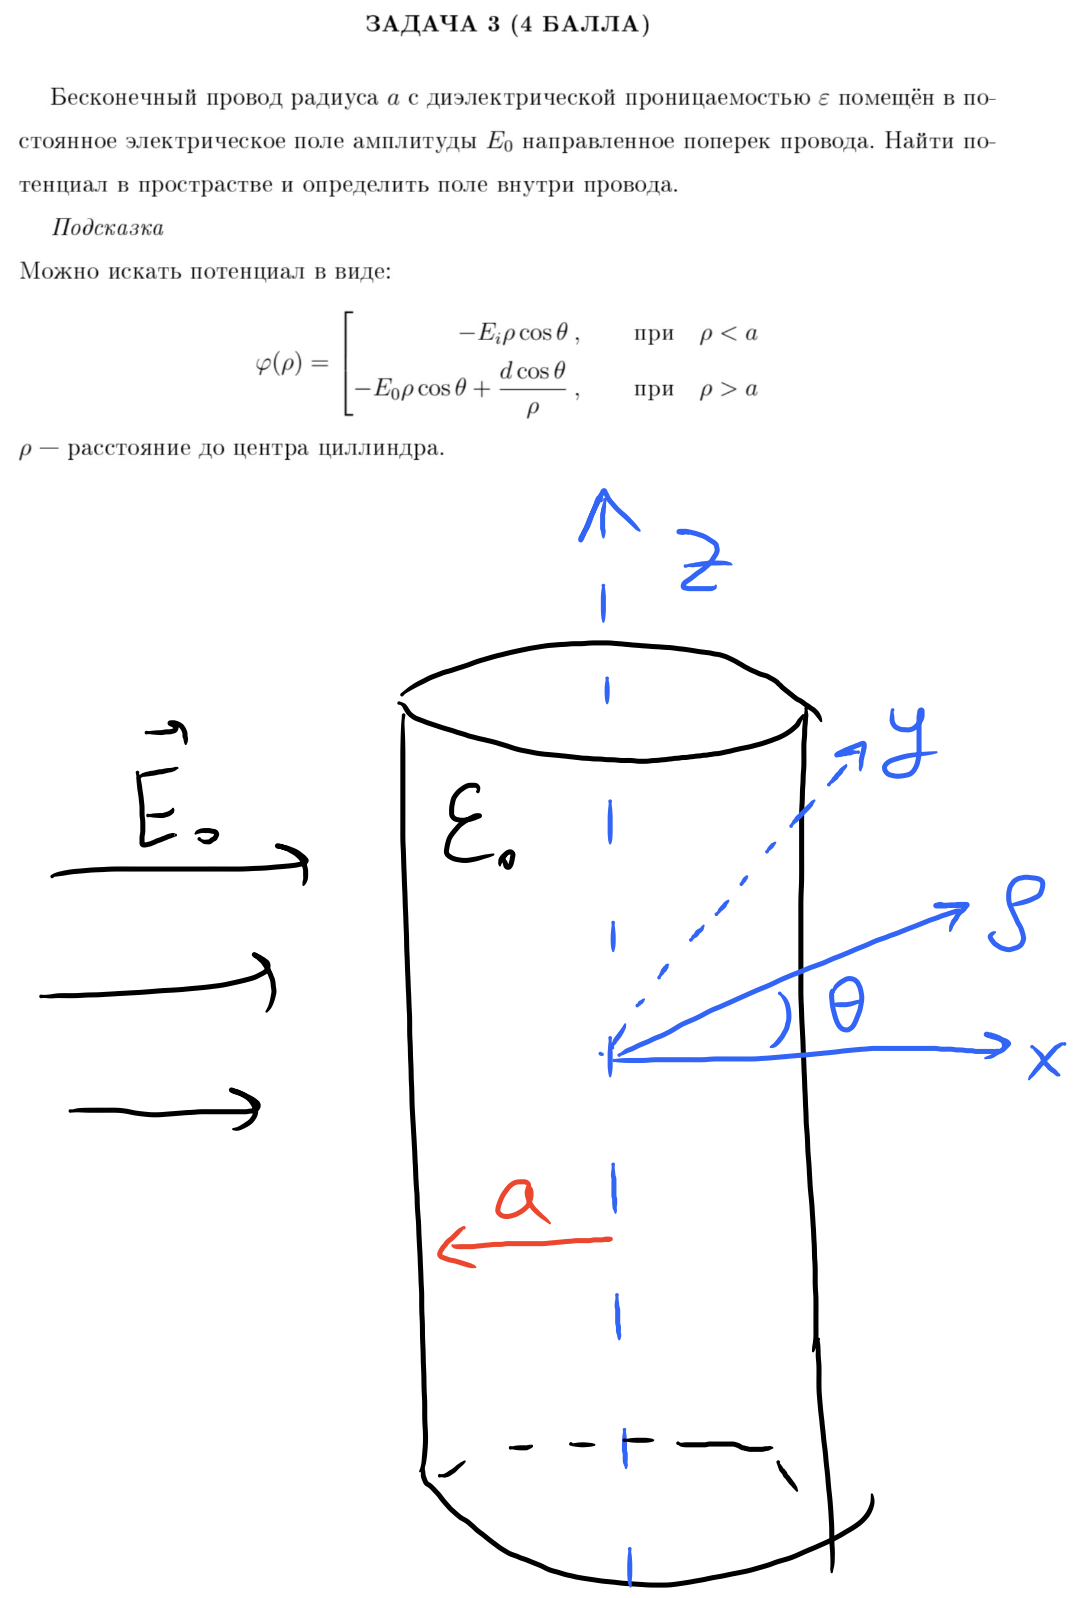
\includegraphics[width=1\textwidth]{photo.png}
%\begin{center}
%\underline{Рисунок 1}:
%\end{center}
\par Решение:
\par
\par Условие генерации второй ТМ гармоники:
\[
    2 \cdot k_{TE}( \omega ) = k_{TM}(2 \omega )
\]
\par
%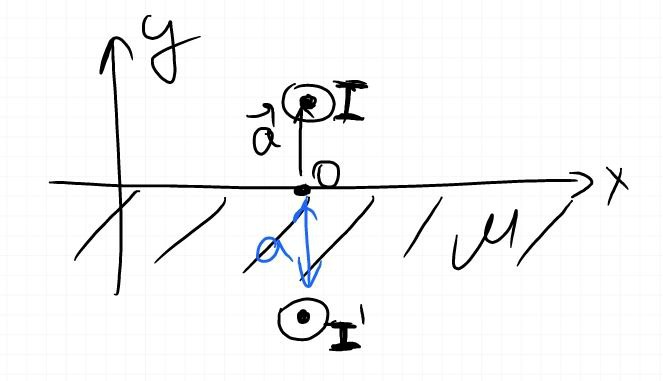
\includegraphics[width=1\textwidth]{photo_1.jpg}
%\par
\begin{center}
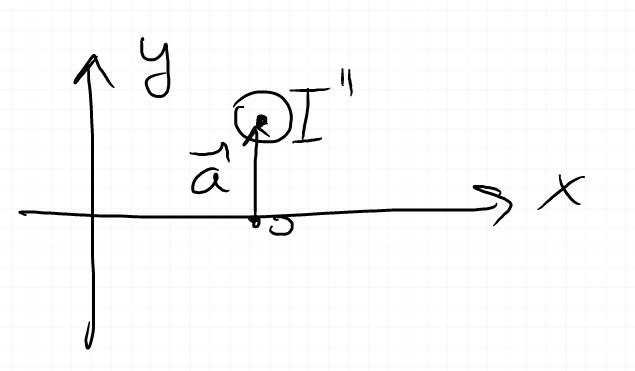
\includegraphics[width=0.4\textwidth]{photo_2.jpg}
\end{center}
\par Дисперсионное соотношение:
\[
    k^2( \omega ) = \varepsilon ( \omega ) \frac{ \omega^2 }{c^2}
\]
\par Так как ТЕ поляризации соответствует обыкновенная волна, то:
\[
    K_{TE}^2 ( \omega ) = \varepsilon_{xx} ( \omega ) \frac{ \omega^2 }{c^2}
\]
\par А для ТМ поляризации:
\[
    K_{TM}^2 ( \omega ) = K_{TM; x}^2 ( \omega ) + K_{TM; z}^2 ( \omega ) = \left( tg^2 \theta + 1 \right) K_{TM; z}^2 ( \omega ) = \frac{\varepsilon_{zz} ( \omega ) \frac{ \omega^2 }{c^2}}{ \cos^2 \theta }
\]
\par Используя условие генерации получаем:
\[
    2 \sqrt{K_{TE}^2 ( \omega )} = \sqrt{K_{TM}^2 ( 2 \omega )}
\]
\[
    2 \sqrt{ \varepsilon_{xx} ( \omega ) \frac{ \omega^2 }{c^2} } = \sqrt{ \frac{\varepsilon_{zz} ( 2 \omega ) \frac{ ( 2 \omega )^2 }{c^2}}{ \cos^2 \theta } }
\]
\[
    \sqrt{\varepsilon_{xx} ( \omega )} = \frac{\sqrt{\varepsilon_{zz} (2 \omega )}}{ \cos \theta }
\]
\[
    \cos \theta = \sqrt{\frac{\varepsilon_{zz} (2 \omega )}{\varepsilon_{xx} ( \omega )}}
\]
\par Ответ:
\[
    \cos \theta = \sqrt{\frac{\varepsilon_{zz} (2 \omega )}{\varepsilon_{xx} ( \omega )}}
\]
\par
\par
\end{large}
\end{document}
